\section{基于LSTM序列模型分类}
目前很多研究表明,深度学习和神经网络在图像识别和自然语言处理(NLP)方面表现出众。我们可以利用神经网络的NLP能力来处理这个分类问题。本方法是利用了Google的Tensorflow这个框架搭建相关模型,用相关数据集来判断此模型的正确率。基于LSTM序列模型分类的恶意URL检测算法如下:
\begin{algorithm}[!ht]
    \SetAlgoNoLine
    % \SetAlgoNoLine可以去掉竖线
    \caption{基于LSTM序列模型分类的恶意URL检测算法}
    \KwIn{URL Text in JSON}
    \KwOut{The Evaluate and Prediction Outputs}
    load data\; 
    preprocess each URL into a sequence of characters\;
    map the each character of the request log text to numeric values within a word dictionary\;
    init a LSTM neural network model\;
    split the data into training set and validating set\;
    start train training set\;
    validate and evaluate the predictions\;
\end{algorithm}
\subsection{预处理数据}
本方法\cite{Sui2010Content}采用\cite{Zhang2013DTU}的文本数据是模拟API给出JSON形式的访问请求日志,样例请看(图\ref{fig:json_sample})。URL文本数据和标签(正常访问还是攻击行为)以|进行切分。对URL文本进行预处理时由于请求日志的内容包含各种字符串、符号和数字,因此,本方法将请求日志文本中的每个字符映射到字典中的数字。相关联的数字表示该字符出现的频率。这个字典是用训练数据来创建的。对于每一条URL,本方法设定固定字符长度为1024,对于小于1024长度的数据部分进行头部padding填充。预处理完毕之后的数据形式如下(图\ref{fig:vec2}):
\begin{figure}[!ht]
    \setlength{\abovecaptionskip}{0.cm}
    \setlength{\belowcaptionskip}{-0.cm}
    \centering
     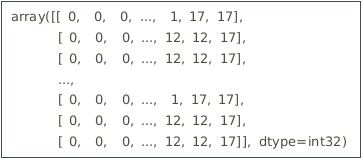
\includegraphics[scale=0.5]{Figs/vec2.png}
    \caption{Json URL向量化后的部分样例}
    \label{fig:vec2}
\end{figure}
\subsection{模型构建}
为了快速开发神经网络模型,本文选择使用运行在Tensorflow之上的高级框架Keras API。通过使用Keras为Tensorflow提供的样板设置,我们能够快速构建起模型原型。
\\\indent{}模型的结构如下(图\ref{fig:LSTM})显示:
\begin{figure}[!ht]
    \setlength{\abovecaptionskip}{0.cm}
    \setlength{\belowcaptionskip}{-0.cm}
    \centering
     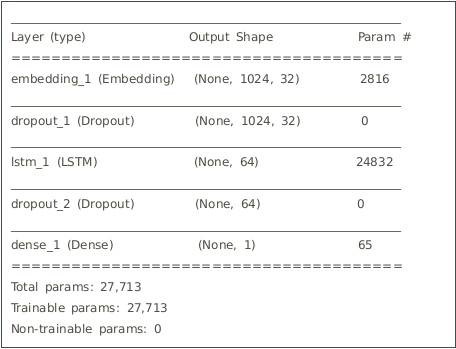
\includegraphics[scale=0.65]{Figs/lstm.png}
    \caption{LSTM模型网络结构}
    \label{fig:LSTM}
\end{figure}
\\\indent{}Sequential Model初始的第一层嵌入层指定了向量输入的预期维度,本文使用嵌入层将预处理过的数据数值进行归一化,并进行Embedding嵌入。
\\\indent{}第二层和第四层Dropout层是将在训练过程中每次更新参数时按一定概率(rate)随机断开输入神经元,用于防止过拟合。
\\\indent{}第三层则是模型主要部分LSTM部分,LSTM隐藏层则由64个神经元以及循环状态的线性变换中神经元断开比例为50\%。
\\\indent{}最后第五层则是全连接层,并用一个sigmoid激活函数进行约束,以产生0\~1之间的分类置信度。
\subsection{训练模型}
得到了LSTM的模型实例和处理过的数据,标签后,需要将数据集分为训练集和测试集。训练集占了所有数据集合的$75\%$,验证集是$25\%$。训练三次,每进行梯度下降时batch包含的样本数为128。最后的训练结果如如下(图\ref{fig:LSTM_train})显示:
\begin{figure}[!ht]
    \setlength{\abovecaptionskip}{0.cm}
    \setlength{\belowcaptionskip}{-0.cm}
    \centering
     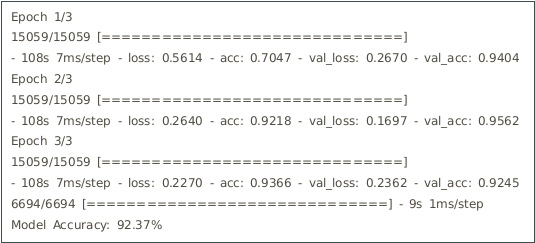
\includegraphics[scale=0.5]{Figs/LSTM_train.png}
    \caption{LSTM模型网络训练结果}
    \label{fig:LSTM_train}
\end{figure}
\subsection{测试模型}
进过训练之后,将模型对另外两个数据集进行测试,得到如下(表\ref{table:lstm_test})测试结果:
\begin{table}[!ht]
    \setlength{\abovecaptionskip}{0.cm}
    \setlength{\belowcaptionskip}{-0.cm}
    \caption{LSTM训练后模型测试结果}
    \centering
    \label{table:lstm_test}    
    \begin{tabular}{|c|c|c|c|}
        \hline
        &json数据&普通URL&FWaf项目\\
        \hline
        Accuracy&0.9216&0.5141&0.8057\\
        \hline
    \end{tabular}
\end{table}
\\\indent{}模型的结果在json数据格式上能过达到95\%以上的正确率,但是用到直接的URL上效果就不是那么好了,可能是数据文本形态的不同所导致的结果。